% !TEX root = ../main.tex
% =====================================================================
% fig_pool_aggregators.tex -- one small panel per MIL pooling head.
%
% Every panel applies that head's aggregator to the SAME made-up evidence
% profile g_j^k, so the panels differ only by the aggregator. That is the
% whole point of the figure: it shows which evidence actually reaches the
% bag score under each head.
%
% Dark orange = counts fully, pale orange = counts a little, grey = dropped.
% Two columns, four rows. Natural width ~13.5 cm, so \resizebox barely
% shrinks it and the labels stay readable.
% =====================================================================

\resizebox{0.82\linewidth}{!}{%
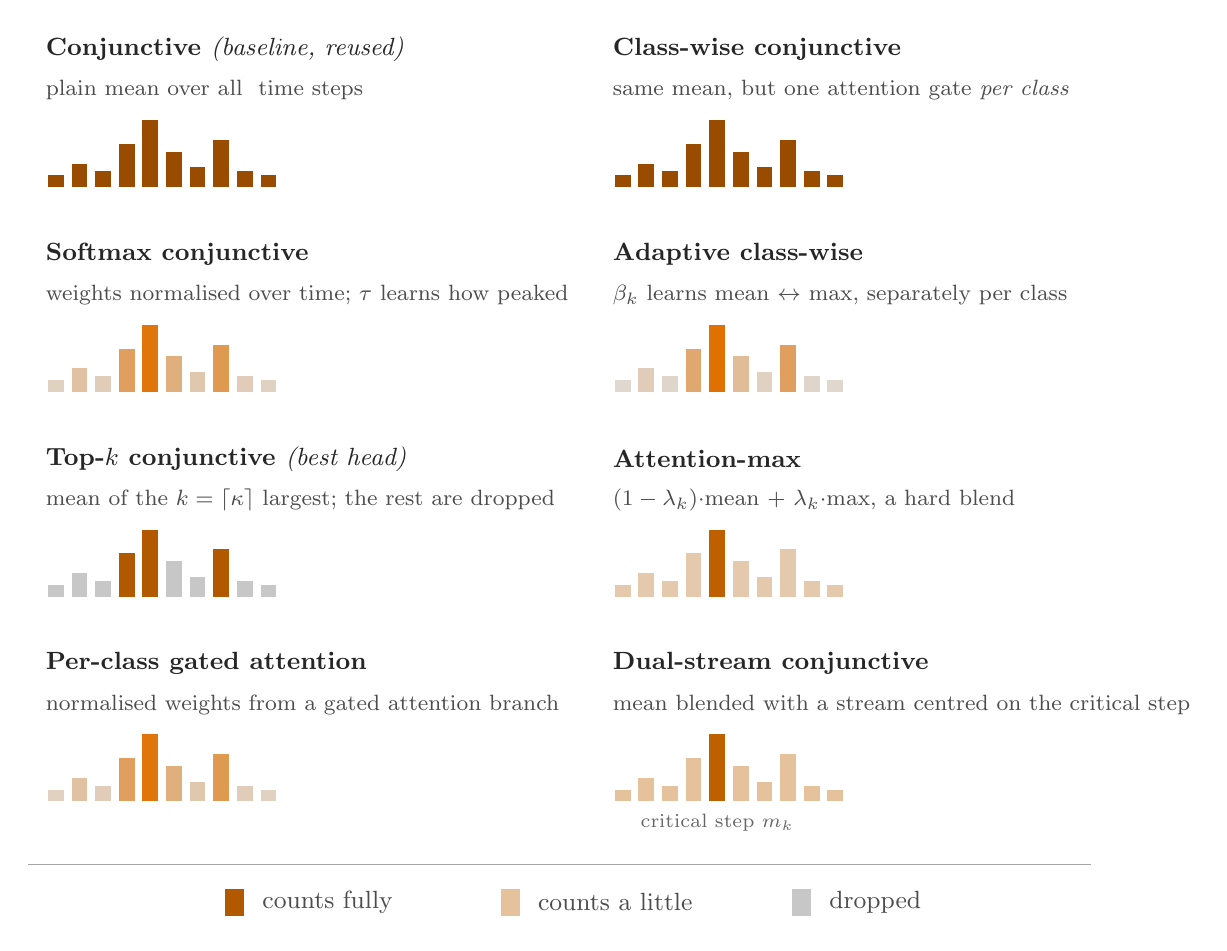
\begin{tikzpicture}[
  font=\small,
  pname/.style = {anchor=west, font=\small\bfseries, black!85, align=left},
  pdesc/.style = {anchor=west, black!70, align=left, font=\footnotesize},
]

% --- one panel: #1 x-shift, #2 y-shift, #3 name, #4 one-line description ----
\def\panelhead#1#2#3#4{%
  \node[pname] at ({#1},{#2})          {#3};
  \node[pdesc] at ({#1},{(#2)-0.52})   {#4};
}

% ============================ row 1 ==================================
\panelhead{0}{0}{Conjunctive \normalfont\itshape (baseline, reused)}
              {plain mean over all $\nsteps$ time steps}
\begin{scope}[shift={(0.15,-1.75)}]
  \foreach \i/\hh in {0/0.15,1/0.30,2/0.20,3/0.55,4/0.85,5/0.45,6/0.25,7/0.60,8/0.20,9/0.15}
    { \fill[orange!60!black] (\i*0.30,0) rectangle ++(0.20,\hh); }
\end{scope}

\panelhead{7.2}{0}{Class-wise conjunctive}
              {same mean, but one attention gate \emph{per class}}
\begin{scope}[shift={(7.35,-1.75)}]
  \foreach \i/\hh in {0/0.15,1/0.30,2/0.20,3/0.55,4/0.85,5/0.45,6/0.25,7/0.60,8/0.20,9/0.15}
    { \fill[orange!60!black] (\i*0.30,0) rectangle ++(0.20,\hh); }
\end{scope}

% ============================ row 2 ==================================
\panelhead{0}{-2.6}{Softmax conjunctive}
              {weights normalised over time; $\tau$ learns how peaked}
\begin{scope}[shift={(0.15,-4.35)}]
  \foreach \i/\hh/\op in {0/0.15/14,1/0.30/28,2/0.20/18,3/0.55/58,4/0.85/95,5/0.45/44,
                          6/0.25/22,7/0.60/64,8/0.20/18,9/0.15/14}
    { \fill[orange!\op!white!88!black] (\i*0.30,0) rectangle ++(0.20,\hh); }
\end{scope}

\panelhead{7.2}{-2.6}{Adaptive class-wise}
              {$\beta_k$ learns mean $\leftrightarrow$ max, separately per class}
\begin{scope}[shift={(7.35,-4.35)}]
  \foreach \i/\hh/\op in {0/0.15/8,1/0.30/18,2/0.20/10,3/0.55/50,4/0.85/100,5/0.45/32,
                          6/0.25/14,7/0.60/58,8/0.20/10,9/0.15/8}
    { \fill[orange!\op!white!88!black] (\i*0.30,0) rectangle ++(0.20,\hh); }
\end{scope}

% ============================ row 3 ==================================
\panelhead{0}{-5.2}{Top-$k$ conjunctive \normalfont\itshape (best head)}
              {mean of the $k=\lceil\kappa\nsteps\rceil$ largest; the rest are dropped}
\begin{scope}[shift={(0.15,-6.95)}]
  \foreach \i/\hh in {0/0.15,1/0.30,2/0.20,5/0.45,6/0.25,8/0.20,9/0.15}
    { \fill[black!22] (\i*0.30,0) rectangle ++(0.20,\hh); }
  \foreach \i/\hh in {3/0.55,4/0.85,7/0.60}
    { \fill[orange!70!black] (\i*0.30,0) rectangle ++(0.20,\hh); }
\end{scope}

\panelhead{7.2}{-5.2}{Attention-max}
              {$(1-\lambda_k)\cdot$mean $+\ \lambda_k\cdot$max, a hard blend}
\begin{scope}[shift={(7.35,-6.95)}]
  \foreach \i/\hh in {0/0.15,1/0.30,2/0.20,3/0.55,5/0.45,6/0.25,7/0.60,8/0.20,9/0.15}
    { \fill[orange!25!white!90!black] (\i*0.30,0) rectangle ++(0.20,\hh); }
  \fill[orange!75!black] (4*0.30,0) rectangle ++(0.20,0.85);
\end{scope}

% ============================ row 4 ==================================
\panelhead{0}{-7.8}{Per-class gated attention}
              {normalised weights from a gated attention branch}
\begin{scope}[shift={(0.15,-9.55)}]
  \foreach \i/\hh/\op in {0/0.15/14,1/0.30/28,2/0.20/18,3/0.55/58,4/0.85/95,5/0.45/44,
                          6/0.25/22,7/0.60/64,8/0.20/18,9/0.15/14}
    { \fill[orange!\op!white!88!black] (\i*0.30,0) rectangle ++(0.20,\hh); }
\end{scope}

\panelhead{7.2}{-7.8}{Dual-stream conjunctive}
              {mean blended with a stream centred on the critical step}
\begin{scope}[shift={(7.35,-9.55)}]
  \foreach \i/\hh in {0/0.15,1/0.30,2/0.20,3/0.55,5/0.45,6/0.25,7/0.60,8/0.20,9/0.15}
    { \fill[orange!32!white!90!black] (\i*0.30,0) rectangle ++(0.20,\hh); }
  \fill[orange!75!black] (4*0.30,0) rectangle ++(0.20,0.85);
  \node[anchor=north, black!60, font=\scriptsize] at ({4*0.30+0.10},-0.04) {critical step $m_k$};
\end{scope}

% ============================ legend =================================
\draw[black!35] (-0.1,-10.35) -- (13.4,-10.35);
\fill[orange!70!black]          (2.4,-11.00) rectangle ++(0.24,0.34);
\node[anchor=west, black!70] at (2.75,-10.83) {counts fully};
\fill[orange!32!white!90!black] (5.9,-11.00) rectangle ++(0.24,0.34);
\node[anchor=west, black!70] at (6.25,-10.83) {counts a little};
\fill[black!22]                 (9.6,-11.00) rectangle ++(0.24,0.34);
\node[anchor=west, black!70] at (9.95,-10.83) {dropped};

\end{tikzpicture}}
